\section{Technischer Hintergrund}
In diesem Abschnitt wird das für die späteren Abschnitte benötigte 
Hintergrundwissen beschrieben. Zuerst wird auf MAC-Adressen (Media Access Control) 
im Allgemeinen eingegangen, dann wird der WLAN Standard genauer beschrieben 
und danach wird auf Details der Probe-Requests eingegangen.

\subsection{MAC-Adressen}
Die Media-Access-Control Adresse ist eine ID zur eindeutigen Identifikation
von Netzwerkcontrollern (NIC, Network Interface Controller), um in einem 
Netzwerk mit anderen Geräten kommunizieren zu können.
Die MAC wird in den meisten Netzwerktechnologien- z.B. Wi-Fi, Bluetooth oder 
Ethernet- verwendet, um sich mit einem Netzwerk zu verbinden und ist einzigartig
für jeden NIC. MAC-Adressen werden von der IEEE (Institute of Electrical and Electronics
Engineers) für jeden Hersteller zugewiesen.

Die MAC-Adresse setzt sich aus sechs Bytes (48 Bit) zusammen und wird vom 
Gerätehersteller in der Manufaktur direkt hartcodiert. 
In der Abbildung~\ref{figure:macadresseaufbau} ist der Aufbau der MAC ersichtlich.
Üblicherweise sind die ersten drei Bytes (24 Bit) die Beschreibung des 
Herstellers, auch Herstellerkennung oder OUI (Organizational Unique Identifier)
genannt.  

\begin{figure}[h!]
	\centering
	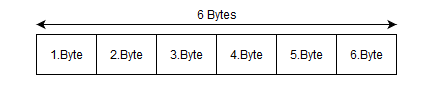
\includegraphics[width=1\linewidth]{Analyse/MACAddressOne.PNG}
	\caption{MAC-Adresse Aufbau
	\label{figure:macadresseaufbau}}
\end{figure}
Die restlichen drei Bytes sind für die Identifikation des NIC reserviert.
Es gibt zwei Bit, beide im ersten Byte der Adresse,
die für die MAC-Adresse eine besondere Relevanz haben.
Das Gruppenbit, welches sich an der letzten Stelle im Byte befindet, 
wird für die Unterscheidung von Unicast- und Multicast-Adressen verwendet.
Das Lokale oder U/L-Bit an der zweitletzten Stelle unterscheidet zwischen
global einzigartigen (und von der IEEE zugewiesenen) Adressen und lokal 
verwalteten Adressen.

\clearpage 

In der Abbildung~\ref{figure:macadressedetail} ist die Struktur der MAC-Adresse dargestellt.
\begin{figure}[h!]
	\centering
	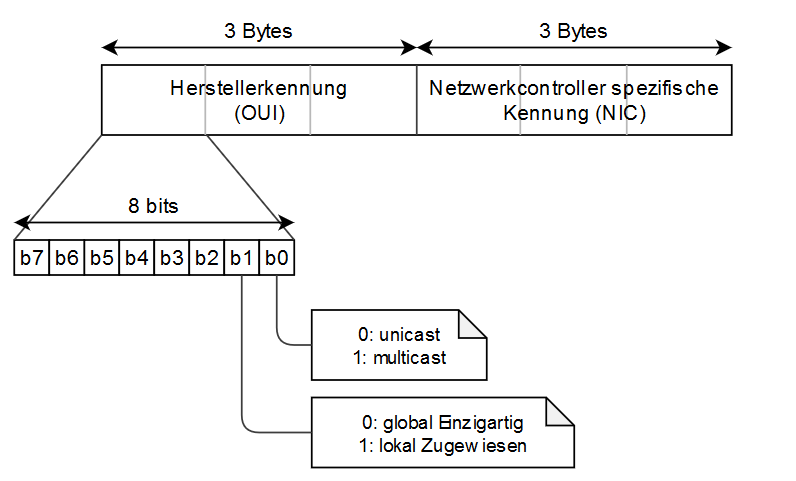
\includegraphics[width=1\linewidth]{Analyse/MACAddressTwo.PNG}
	\caption{Detaillierte MAC-Adresse
	\label{figure:macadressedetail}}
\end{figure}

Falls das lokale Bit gesetzt ist, kann dies anhand der MAC-Adresse sehr schnell
erkannt werden, da das zweite Zeichen im ersten Byte eine von vier Zahlen 
gemäss der Tabelle~\ref{table:localmacrange} ist.

\begin{table}[h!]
	\centering
	\begin{tabular}{|c|}
		\hline
		x2-xx-xx-xx-xx-xx \\
        \hline
        x6-xx-xx-xx-xx-xx \\
        \hline
        xA-xx-xx-xx-xx-xx \\
        \hline
        xE-xx-xx-xx-xx-xx \\
        \hline
    \end{tabular}
    \caption{Lokale MAC-Adressen
    \label{table:localmacrange}}  
\end{table}

\clearpage

\subsection{IEEE 802.11 WLAN Standard}
Der IEEE 802.11 Standard ist eine Ansammlung von Protokollen, 
die das Zusammenspiel von Komponenten in kabellosen Netzwerken 
(WLAN, Wireless Local Area Network) regeln, und baut auf dem 802 Standard
Für lokale Computernetzwerke (LAN) auf.

Der WLAN Standard definiert unter anderem 
auf welche Art und Weise Computer, Mobiltelefone und andere Geräte 
miteinander interagieren welche Frequenzbänder sie dabei verwenden, 
welche Formate die übertragenen Datenpakete haben müssen und welche 
Sicherheitsvorkehrungen getroffen werden sollen.

Nachfolgend wird auf die wichtigsten Spezifikationen und Konzepte eingegangen, 
die im Rahmen dieser Arbeit relevant sind.

\subsubsection*{Frequenzbänder}
Die meistverwendeten Frequenzbänder im WLAN sind das $2.4$-GHz-Band und das 
$5$-GHz-Band. Diese Frequenzbänder sind jeweils in gleich grosse Kanäle 
unterteilt.
Um Störungen durch überlappende Frequenzbänder zu verhindern, werden 
im $2.4$-GHz-Bereich in Europa üblicherweise die Kanäle $1$, $6$ und $11$ 
verwendet.
In der Abbildung~\ref{figure:lowerfrequencyband} ist die Unterteilung der 
Kanäle ersichtlich.
Im $5$-GHz-Bereich wird die Kanalunterteilung in Europa gemäss der 
Tabelle~\ref{table:higherfrequencyband} vorgenommen.

\begin{figure}[h!]
	\centering
	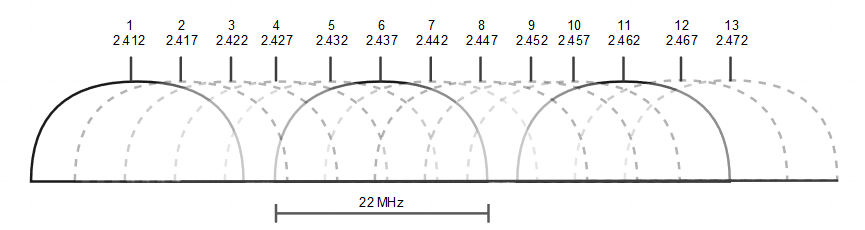
\includegraphics[width=1\linewidth]{Analyse/lowerfrequencyband.PNG}
	\caption{Kanalzuteilung im $2.4$-GHz-Frequenzband
	\label{figure:lowerfrequencyband}}
\end{figure}

\clearpage

\begin{table}[h!]
	\centering
	\begin{tabular}{|>{$}c<{$}|>{$}c<{$}||>{$}c<{$}|>{$}c<{$}|}
		\hline
        \textbf{Kanal} & \textbf{Frequenz} & \textbf{Kanal} & \textbf{Frequenz} \\
        \hline
        \phantom{0}36 & 5,180 & 108 & 5,540 \\ 	
        \phantom{0}40 & 5,200 & 112 & 5,560 \\
        \phantom{0}44 & 5,220 & 116 & 5,580 \\
        \phantom{0}48 & 5,240 &	120 & 5,600 \\
        \phantom{0}52 & 5,260 & 124 & 5,620 \\
        \phantom{0}56 & 5,280 & 128 & 5,640 \\
        \phantom{0}60 & 5,300 & 132 & 5,660 \\
        \phantom{0}64 & 5,320 & 136 & 5,680 \\
        100 & 5,500 & 140 & 5,700 \\
        104 & 5,520 & &\\	
        \hline
    \end{tabular}
    \caption{Kanalzuteilung $5$-GHz-Frequenzband. Jeder Kanal ist $20$ MHz breit. 
    \label{table:higherfrequencyband}}  
\end{table}


Geräte, die über das WLAN kommunizieren, werden auf die Kanäle aufgeteilt, 
so dass alle Kanäle gleichmässig ausgelastet sind, 
um eine möglichst grosse Datenrate für jedes Endgerät zu gewährleisten.
Somit ist es nicht möglich, nur einen Kanal zu überwachen, um sämtliche
Endgeräte in einem WLAN-Netzwerk zu identifizieren.

\clearpage

\subsection{802.11 Frames}
Im IEEE 802.11 Standard ist definiert, wie die Datenpakete, 
sogenannte Frames, aufgebaut sein müssen.
Diese Frames befinden im OSI-Modell (Siehe Abbildung~\ref{figure:ozzylayer}) 
auf dem zweiten Layer, dem Data Link Layer \\ (Sicherungsschicht).

\begin{figure}[h!]
	\centering
	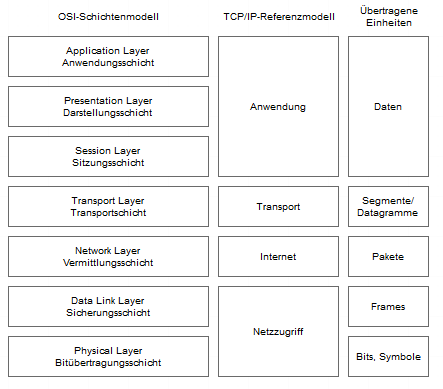
\includegraphics[width=1\linewidth]{Analyse/ozzylayer.PNG}
	\caption{OSI- und TCP/IP-Referenzmodell
	\label{figure:ozzylayer}}
\end{figure}

\clearpage

Frames können in drei Kategorien unterteilt werden:

Datenframes, welche Daten von höheren Schichten übertragen, 
z.B. TCP-Segmente aus der Transportschicht.

Control-Frames, die bei der Übertragung der Datenframes den Kontrollfluss
steuern und die Zuverlässigkeit der WLAN-Übertragung gewährleisten. \\
Beispiele für Control-Frames sind Request-To-Send- oder Acknowledgment-
Nachrichten.

Die dritte Kategorie sind die Management-Frames, welche verschiedene
Dienste auf dem Data Link Layer für WLAN anbieten, die im Kabelgebundenen
LAN nicht benötigt werden. Ein Beispiel hierfür wäre die Identifizierung von verfügbaren 
Netzwerken.
Die in dieser Arbeit untersuchten Probe-Requests gehören in diese dritte Kategorie.
In der Abbildung~\ref{figure:genericmanagementframe} ist ein Management- 
Frame dargestellt, wie es üblicherweise versendet wird. 
Die MAC-Header-Informationen sind in jedem Frame enthalten, aber die 
Information Elements können sich je nach Typ des Management-Frames unterscheiden.
Eine Erklärung der einzelnen Felder ist in der 
Tabelle~\ref{table:genericmanagementframe} angegeben.

\begin{figure}[h!]
	\centering
	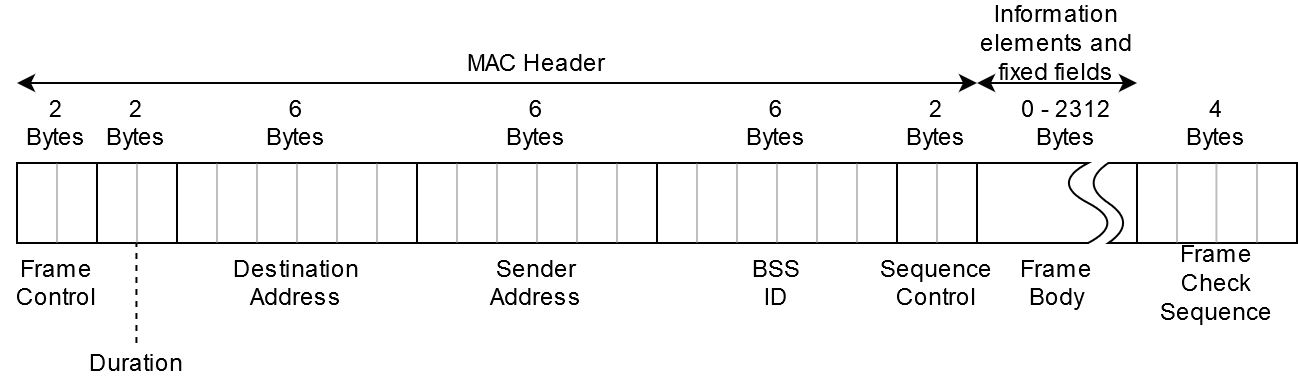
\includegraphics[width=1\linewidth]{Analyse/GenericManagementFrame.png}
	\caption{Generisches Management-Frame
	\label{figure:genericmanagementframe}}
\end{figure}

\begin{table}[h!]
	\centering
	\begin{tabular}{|c|>{$}c<{$}|l|}
		\hline
        \textbf{Feld} & \textbf{Länge} & \textbf{Bedeutung} \\
        \hline
        Frame Control & 2\, \text{Byte} & 
        Gibt die Protokollversion und Subtype- \\
        & & Informationen für das Frame an. \\
        \hline
        Duration & 2\, \text{Byte} & 
        Gibt die Zeit an, wie lange das Übertragungs- \\
        & & medium während der Übertragung des Frames \\
        & & nicht verwendet werden darf, um Kollisionen  \\
        & & zu vermeiden. \\
        \hline 
        Dest. Address & 6\, \text{Byte} & 
        MAC-Adresse des Empfängers des Frames. \\
        \hline 
        Sender Address & 6\, \text{Byte} & 
        MAC-Adresse des Sendegeräts des Frames. \\
        \hline
        BSSID & 6\, \text{Byte} & 
        BSSID steht für Basic Service Set Identifier \\
        && und beschreibt eine Zuordung verschiedener \\
        && Geräte zu einem spezifischen Netzwerk. \\
        && Üblicherweise ist die BSSID die MAC- \\
        && Adresse des Access Points \\
        \hline
        Sequence Control & 2\, \text{Byte} & 
        Dieses Feld besteht aus einer Fragmentnummer\\
        && und einer Sequenznummer. \\
        && Die Fragmentnummer beschreibt die Anzahl \\
        && Frames, die für einen Request benötigt werden. \\
        && Die Sequenznummer wird für jede Übertragung \\
        && separat festgelegt und verwendet, falls \\
        && Übertragungen wiederholt werden müssen. \\
        \hline
        Frame-Body & \text{variabel} & 
        Im Frame-Body werden die spezifischen \\
        && Informationen des jeweiligen Frames \\
        && übertragen. \\
        \hline
        Frame Check Sequence & 2\, \text{Byte} & 
        Redundanzcheck für die Validierung, dass \\
        && das Frame korrekt übertragen wurde. \\
        \hline
    \end{tabular}
    \caption{Felder in einem Management-Frame
    \label{table:genericmanagementframe}}  
\end{table}

\clearpage 

Weiterhin können Frames in drei verschiedene Klassen unterteilt werden.
Die Klassen bestimmen, welche Frames - abhängig vom Zustand des Geräts - 
überhaupt übertragen werden dürfen.
Die verschiedenen Zustände und die dazugehörigen erlaubten Klassen sind 
in der Abbildung~\ref{figure:proberequeststate} dargestellt.
Im initialen Zustand sind Geräte nicht authentifiziert und nicht einem
Access Point zugeordnet. 
Im zweiten Zustand hat sich das Gerät gegenüber dem Access Point authentifiziert,
ist aber noch nicht zugewiesen.
Im dritten Zustand ist das Gerät authentifiziert und zugewiesen.
Erst im dritten Zustand ist der Austausch von Daten erlaubt.

\begin{figure}[h!]
	\centering
	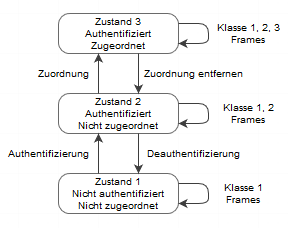
\includegraphics[width=0.8\linewidth]{Analyse/proberequeststate.PNG}
	\caption{Zustände und Klassen für Frames
	\label{figure:proberequeststate}}
\end{figure}

\clearpage

\subsection{Probe-Requests}
Probe-Requests sind Klasse-1 Management-Frames. Sie werden von End-geräten 
verwendet, um innerhalb des Sendebereiches nach WLAN-Access-Points zu suchen. 
Alternativ können Netzwerke auch gefunden werden, 
indem ausgesendete Beacon-Messages der Access Points empfangen werden.
Um sich mit einem Access Point zu verbinden, sendet ein Gerät zuerst 
Probe-Requests als Broadcast aus, um verfügbare Access Points kennen zu lernen.
Alle Access Points im Sendebereich des Geräts, die den Request erhalten,
senden eine Probe-Response, um die vom Gerät benötigten Parameter 
und die eigenen Betriebsparameter zu übermitteln. 
Das Gerät evaluiert die erhaltenen Responses, wählt für sich den 
besten Access Point aus und sendet diesem einen Auth.-Request
mit den für die Authentifizierung be-nötigten Informationen. Sind diese 
Informationen für den Access Point korrekt, sendet dieser
ein Auth.-Response und registriert das Gerät bei sich.
Das Gerät sendet daraufhin einen Association-Request welcher vom Access
Point mit einem Association-Response beantwortet wird, bevor dann der 
Austausch von Daten zwischen Endgerät und Access Point beginnt.
Der gesamte Ablauf ist in der Abbildung~\ref{figure:proberequestsequence} 
dargestellt.

\begin{figure}[h!]
	\centering
	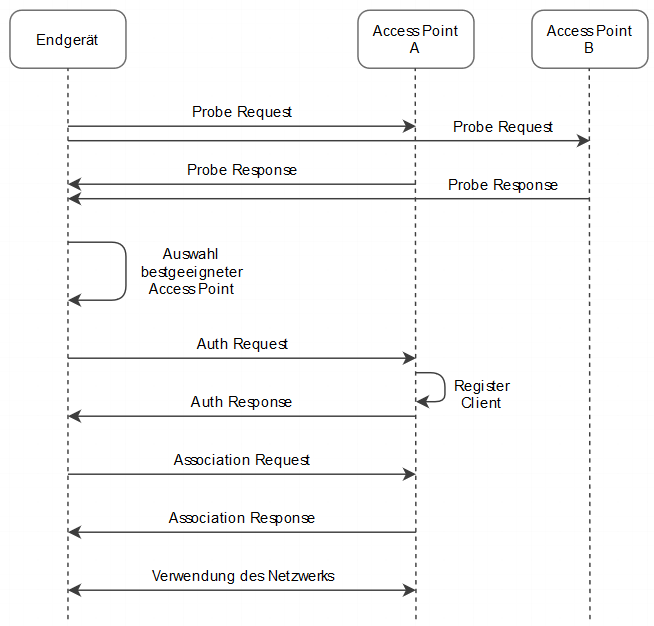
\includegraphics[width=0.8\linewidth]{Analyse/proberequestsequence.PNG}
	\caption{Sequenzdiagramm Association und Authentifizierung
	\label{figure:proberequestsequence}}
\end{figure}

Probe-Requests beinhalten alle notwendigen Informationen, die ein Access Point
benötigt, um zu entscheiden, ob er die Anforderungen des Client-Geräts 
erfüllen kann. In der Abbildung~\ref{figure:proberequestframe} ist das Frame
eines Probe-Requests ersichtlich und in der Tabelle~\ref{table:proberequestframe}
sind die einzelnen Felder erklärt.

\begin{figure}[h!]
	\centering
	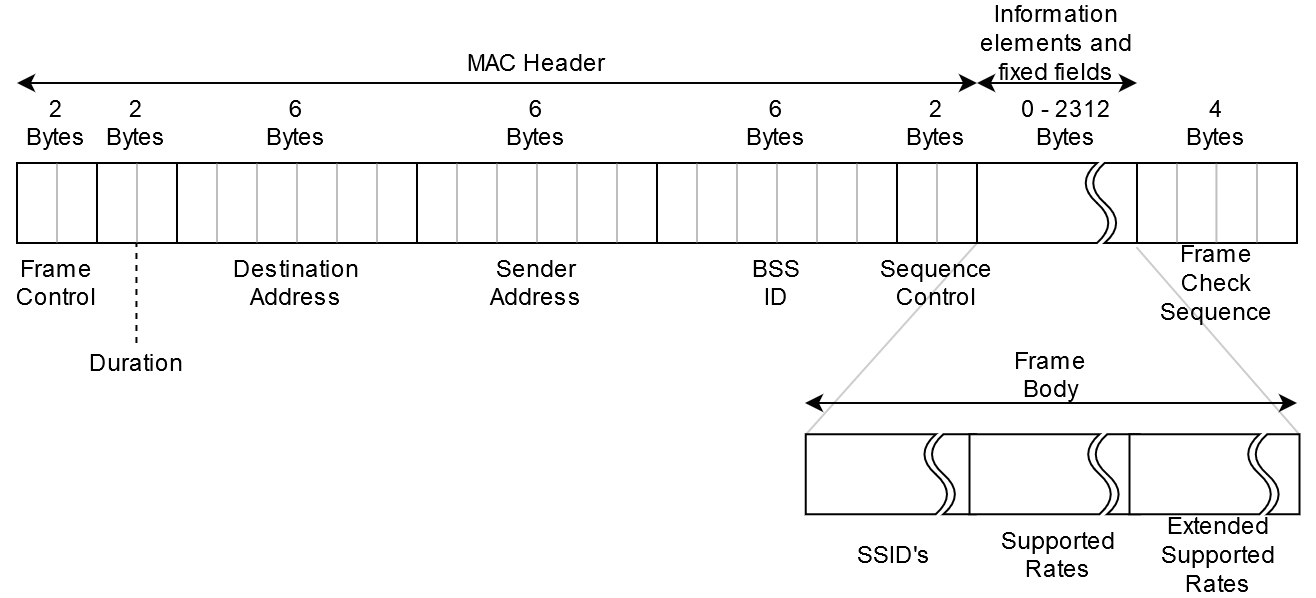
\includegraphics[width=1\linewidth]{Analyse/ProbeRequestFrame.png}
    \caption{Frame eines Probe-Requests.
	\label{figure:proberequestframe}}
\end{figure}

\begin{table}[h!]
	\centering
	\begin{tabular}{|c|c|l|}
		\hline
        \textbf{Feld} & \textbf{Länge} & \textbf{Bedeutung} \\
        \hline
        SSID & variabel & 
        Abfolge von Zeichen, um ein Netzwerk zu \\ 
        && identifizieren. \\
        && Wird manchmal auch als Netzwerkname bezeichnet. \\
        \hline
        (Extended) & variabel & 
        Datenraten, die vom Client-Gerät unterstützt werden. \\
        Supported Rates & & 
        Im IEEE 802.11 sind verschiedene Datenraten von \\
        && 1Mbit/s bis 54MBit/s standardisiert. \\
        \hline
    \end{tabular}
    \caption{Felder in einem Probe-Request
    \label{table:proberequestframe}}  
\end{table}



\clearpage

\subsection{Probe-Request-Burst}
Mobilgeräte senden Probe-Requests in Gruppen aus, welche Bursts genannt werden. 
Bursts zeichnen sich dadurch aus, dass jeder Probe-Request darin dieselbe MAC-Adresse 
verwendet. Die Anzahl Probe-Request kann dabei von Burst zu Burst variieren.
 Weiterhin sind die Sequenznummern innerhalb eines Bursts aufsteigend, 
auch wenn die Sequenznummer vom Mobilgerät zufallsgeneriert sind.
Die Information-Element-Felder der Probe-Requests  in einem Burst sind ebenfalls 
identisch.

Diese Information kann in einem Prototyp dazu verwendet werden, aufgezeichnete 
Frames in Bursts zu sortieren, bevor diese klassifiziert werden.
Da-durch müssen weniger einzelne Frames klassifiziert werden und die Effizienz eines 
Prototyps wird gesteigert, während die Fehlerrate gesenkt wird.

Die Abbildung~\ref{figure:burstcolor} zeigt eine Aufzeichnung von Probe-Requests, 
und wie deren Aufteilung in Bursts erkannt werden kann.

\begin{figure}[h!]
	\centering
	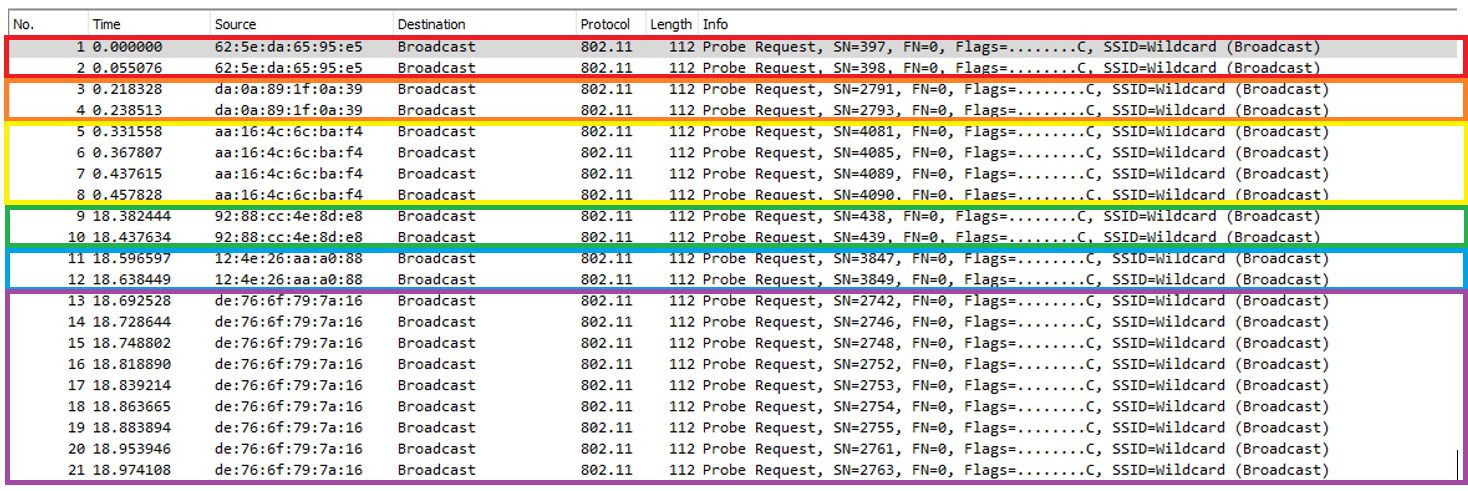
\includegraphics[width=1\linewidth]{Analyse/Burst_Explanation_with_Lines.PNG}
    \caption{Wireshark-Aufzeichnung von Probe-Requests. 
    Die Bursts sind farbig gekennzeichnet.
	\label{figure:burstcolor}}
\end{figure}

Die Probe-Requests in dieser Abbildung stammen alle vom selben Gerät. 
Man kann erkennen, dass die MAC-Adresse und Sequenznummer für jeden Burst neu 
zufallsgeneriert wird und dass die Frames alle dieselbe Länge haben, 
was bedeutet, dass sie die selben Information-Element-Felder haben.

\clearpage

\subsection{Probe-Request Header-Frame}
Der MAC-Header in einem Probe-Request hat einige für Fingerprinting 
interessante Felder. 
Bevor die MAC-Adresse zufällig gesetzt wurde, 
konnte ein Client-Gerät einfach anhand der Sendeadresse erkannt und verfolgt 
werden.
Seit einigen Android/iOS-Versionen werden diese Adressen aber zufallsgeneriert.
Die Felder, welche für ein Fingerprinting genutzt werden können, werden
nachfolgend genauer erläutert:

\subsubsection*{Frame Control} 
Das Feld enthält die in der Tabelle~\ref{table:framecontrolattributes}
beschriebenen Attribute.

\begin{table}[h!]
	\centering
	\begin{tabular}{|c|c|l|}
		\hline
        \textbf{Attribut} & \textbf{Länge} & \textbf{Bedeutung} \\
        \hline
        Protokoll & 2 bit & 
        Dieses Attribut unterscheidet verschiedene WLAN- \\
        Version && Standards. \\
        && Falls ein WLAN-2-Standard entwickelt würde, \\
        && kann dies in der Protokoll Version vom aktuellen \\
        && Standard unterschieden werden. \\
        \hline
        Type & 2 bit & 
        Das Type-Attribut unterscheidet zwischen Control-, \\
        && Daten- und Management-Frames \\
        \hline
        Subtype & 4 bit & 
        Der Subtype unterscheidet die verschiedenen Frames \\
        && zusätzlich. \\
        && Probe-Requests haben den Subtype 4 (0b0100) \\
        \hline
        To DS & 1 bit & 
        Wird gesetzt, wenn das Frame von einem Client- \\
        && Gerät zum Access Point gesandt wird. \\
        \hline
        From DS & 1 bit &
        Wird gesetzt, wenn das Frame vom Access Point zum \\
        && Client-Gerät gesandt wird. \\
        \hline 
        More & 1 bit & 
        Wird gesetzt, falls bei Datenframes die Daten in \\
        Fragments && mehreren Fragmenten übertragen werden.\\
        \hline
        Retry & 1 bit & 
        Falls ein Frame nochmals gesendet werden muss,\\
        &&  weil ein Fehler passiert ist, wird dieses Bit\\
        &&  auf 1 gesetzt. \\
        \hline 
        Power & 1 bit & 
        Akkubetriebene Geräte signalisieren mit diesem  \\
        Management &&  
        Attribut, dass sie nach dem Versenden des Frames\\
        && in den Energiesparmodus  wechseln und der\\
        && Access Point allfällige Antworten zwischen-\\
        && speichern soll. \\
        \hline
        More Data & 1 bit & 
        Falls ein Access Point Daten für ein Client-Gerät \\
        && zwischenspeichert, dann wird dieses Attribut \\
        && gesetzt, um zu indizieren, dass das Frame für \\
        && ein Gerät im Ruhemodus gedacht ist. \\
        \hline
        WEP & 1 bit & 
        Dieses Attribut indiziert, dass der Frame-Inhalt \\
        && verschlüsselt übertragen wird.\\
        \hline
        Order & 1 bit & 
        Wenn dieses Attribut gesetz ist, dann werden Frames \\
        && und dazugehörige Fragmente in der korrekten \\
        && Reihenfolge übertragen. \\
        \hline
    \end{tabular}
    \caption{Attribute im Frame-Control-Feld
    \label{table:framecontrolattributes}}  
\end{table}

In Probe-Requests sind die meisten Attribute auf 0b0 gesetzt.
Das Protokoll-Version-Attribut und der der Typ (Management) sind auch auf 
0b0 und der Subtyp auf 0b0100 (4: Probe-Request) gesetzt.

Diese Informationen können für die Filterung von aufgezeichneten Probe-Requests
verwendet werden, sind in der Unterscheidung von verschiedenen Geräten aber 
nicht relevant.

\subsubsection*{Duration}
Das Duration-Feld wird unter anderem dazu verwendet, dem Empfänger 
mitzuteilen, wie lange die Übertragung für das aktuelle Frame etwa 
dauern wird. Bei Probe-Requests beträgt die geschätzte Zeit Null Mikrosekunden.
Daher lässt sich das Duration-Feld für Fingerprinting auch nicht verwenden.

\subsubsection*{Destination Address}
Die Empfängeradresse bei Probe-Requests ist üblicherweise die Broadcast-Adresse 
(ff:ff:ff:ff:ff:ff). Auch dieses Feld lässt sich für Fingerprinting nicht 
verwenden.

\subsubsection*{Sender Address}
Die MAC-Adresse des Absenders ist, vorausgesetztd die richtigen Geräte-einstellungen
sind gesetzt, randomisiert. Es ist möglich, dass nur die NIC (Netzwerkcontroller 
spezifische Kennung) zufällig gesetzt wird, oder dass die gesamte 
MAC-Adresse randomisiert ist. Dieses Verhalten soll in der Bachelorarbeit 
ermittelt werden.

\clearpage

\subsubsection*{BSSID}
Basic Service Sets werden vergeben, um verschiedene WLAN-Netze im selben 
Gebiet untereinander zu unterscheiden.
Wie bei der Empfängeradresse wird in Probe-Requests für die BSSID auch die 
Broadcast-Adresse \\ (ff:ff:ff:ff:ff:ff) verwendet und kann für ein Fingerprinting nicht verwendet 
werden.

\subsubsection*{Sequence Control}
Das Sequence Control Feld hat zwei Attribute. 
Die Fragmentnummer wird verwendet, um Datenframes, die zu gross sind und in 
einzelne Fragmente aufgeteilt werden, in die korrekte Reihenfolge zu sortieren.
Die Sequenznummer dient der Identifikation der logischen Abfolge von Frames.
Fragmentierte oder wiederholt gesendete Frames haben die gleiche Sequenznummer. 
Die Sequenznummer würde sich für ein Fingerprinting eignen, falls sie nicht
bei neuen Probe-Requests jedes Mal zufällig gesetzt wird. 

\subsubsection*{SSID}
In Probe-Request-Frames wird das SSID Field verwendet, um ein Probe-Request zu einem
spezifischen Access Point (z.B. Eduroam) zu senden. 
Falls der Probe-Request an alle verfügbaren Netzwerke versendet wird, wird die
Broadcast-SSID, manchmal auch Wildcard-SSID genannt, verwendet.
Spezifische SSIDs können für ein Fingerprinting interessant sein.
Wenn ein Client-Gerät in verschiedenen Netzwerken Probe-Requests an dieselbe SSID
sendet, kann das Gerät, falls keine weiteren Geräte nach dieser SSID suchen,
erkannt werden. 

\subsubsection*{(Extended)-Supported-Rates}
Mit dem (Extended)-Supported-Rates Feld teilt das Client-Gerät dem Access Point
mit, welche WLAN-Datenraten unterstützt werden. 
Der Access Point entscheidet unter anderem anhand dieser Datenraten, 
ob er dem Client-Gerät einen Probe-Response senden wird.
Die unterstützten Datenraten könnten für eine Erkennung von Geräten genutzt werden.

\clearpage 

\subsubsection*{Frame Check Sequence}
Die Frame Check Sequence ist eine 32 Bit lange hexadezimale Zahl, die anhand
der im Frame gesetzten Parameter berechnet wird und eine Überprüfung der 
Frames beim Empfänger ermöglicht. Wird ein Frame empfangen, kann der Empfänger
die Frame Check Sequence über das Frame berechnen und diese mit dem im Frame
mitgelieferten Wert vergleichen. Falls die beiden Werte nicht übereinstimmen,
wird das Frame verworfen, oder allenfalls neu angefordert.
Die Frame Check Sequence lässt sich nicht für ein Fingerprinting verwenden.

\subsubsection*{Weitere Information-Element-Felder}
Es ist möglich, dass neben den vorgehend erwähnten Feldern im Frame, 
welche alle vorhanden sein müssen, noch optionale Information-Element-Felder
übermittelt werden, um weitere Funktionalitäten abzudecken oder weitere
Eigenschaften des Client Geräts zu übermitteln.
Diese IE-Felder sind für das Fingerprinting wahrscheinlich die interessanteste
Quelle von Informationen, wenn diese sich von Mobilgerät zu Mobilgerät 
tatsächlich unterscheiden.

\clearpage
